% this file is called up by thesis.tex
% content in this file will be fed into the main document

\chapter{Evaluation}\label{chap:evaluation} % top level followed by section, subsection
In this chapter we will present the results found by our framework, and some challenges we encountered during the gathering of the results.

\section{Setup}
We ran the framework on Ubuntu 18.04 LTS inside a QEMU virtual environment with 62 CPU cores on an AMD ThreadRipper 2990WX processor with 64GB of RAM on which we also compiled the binaries and collected the traces.

We compiled every binary 5 times, twice with the modified Angora compiler, namely one for the fast instrumentation and one with the track instrumentation, once with the \texttt{SymCC} compiler, once with the Fuzz Checker compiler to create the Oracle and once with the static analysis pass.

We collected the traces by letting the fuzzer run for 8 hours on all 62 cores. Then we gave every strategy a maximum of 15 seconds of execution time per condition in a trace. We have chosen this limit because even the ConcolicStrategy could often finish within this time. For the ConcolicStrategy, we give it 13 seconds to calculate the possible executions and the last 2 seconds can be used to try the generated inputs. The execution time of the target binary is included in the execution time of a strategy, since the total time is the time one is interested in when trying to implement the most efficient strategy. The strategies which use randomness, like the RandomTaintStrategy, RandomStrategy and GradientDescentStrategy are executed 5 times, and then the average time to flip is computed for every condition. If any of the 5 runs managed to flip a condition, the condition is set to flipped. We took 5 runs to calculate the average, because of timing constraints.


\section{Results}
In this Section we will show per target binary the effectiveness of a strategy. First we will look at the performance of the strategy by looking at the percentage of flipped conditions and by ranking the strategies by the time it took to flip conditions. We will also inspect the substrategies for the strategies which used these. Then we will inspect the results of the microbenchmarks to see when a strategy fails to flip a branch. After this, we will inspect the collected metrics of the branches and try to find any relation between the performance and these metrics.

\subsection{Flipped conditions}
Since coverage in increased then conditions are flipped, one of the most important measures of performance is the number of flipped conditions. In Figure \ref{fig:flipped-conditions} we show the percentage of flipped conditions out of the total tried conditions per strategy and per program. Since all strategies except the RandomStrategy only work on conditions with taint information, we also added a separate column of the conditions flipped by the RandomStrategy which have taint information available to better compare the results.

\begin{figure}[H]
    \centering
    % include first image
    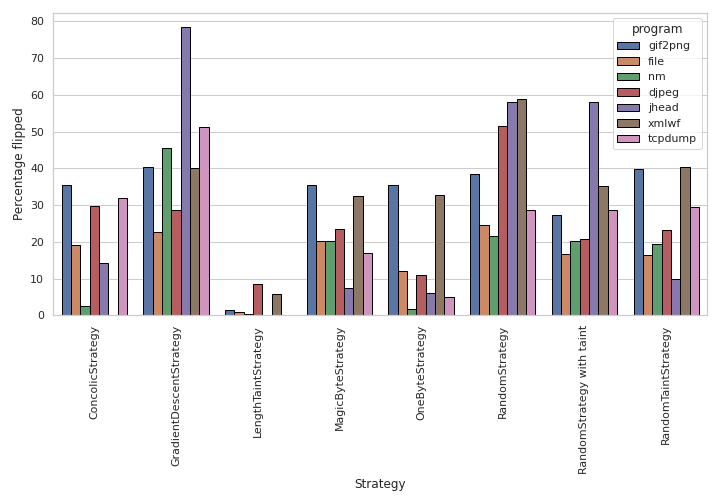
\includegraphics[width=0.8\textwidth]{5_results/graphs_new/percentage_flipped_total.png}  
    \caption{Percentage of all flipped conditions per program}
    \label{fig:flipped-conditions}
\end{figure}

We see that there is quite some difference between the performance of a strategy per program. It appears that the GradientDescentStrategy outperforms the RandomStrategy with taint in most cases, while the LengthTaintStrategy underperforms most other strategies. We also notice that the number of conditions which are flipped by the RandomStrategy with and without taint differ quite a bit per program. Between the \texttt{xmlwf} binary and the \texttt{djpeg} binary, there is a large decrease in the percentage of flipped conditions when only conditions with taint are considered. This looks like the RandomStrategy sometimes flips a lot of conditions which do not have taint information.

We also want to compare the individual conditions. We inspect if there is overlap between the flipped conditions by comparing every strategy with every other strategy. We first take the set of all flipped conditions by one strategy as superset. Then we take all flipped conditions from another strategy as subset and compare how much of the subset is present in the superset. The results are visible in Figure \ref{fig:overlap-strategies}.

\begin{figure}[H]
    \centering
    % include first image
    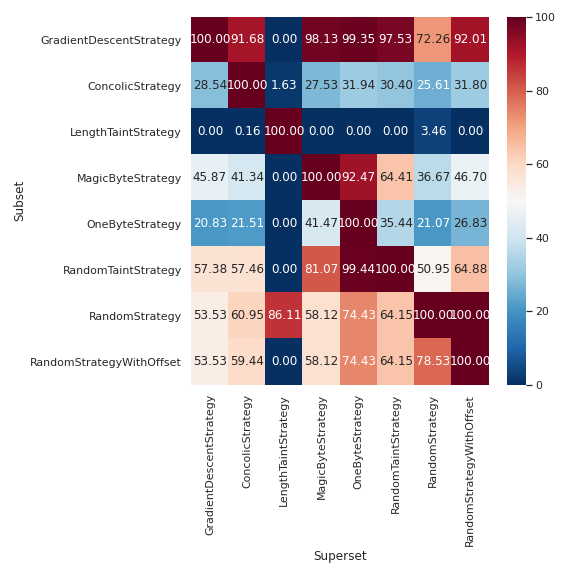
\includegraphics[width=0.75\textwidth]{5_results/graphs_new/overlap_strategies.png}  
    \caption{Percentage of overlap between the super and subset.}
    \label{fig:overlap-strategies}
\end{figure}

Here we notice that for nearly every strategy more than 90\% the flipped conditions are also found by the GradientDescentStrategy. The exception is the LengthTaintStrategy and when only considering the RandomStrategy when also looking at conditions with no taint. From this we expect that the GradientDescentStrategy is a good strategy when trying to flip conditions where taint information is available, and that the RandomStrategy is useful when trying condition when no taint information is available. The LengthTaintStrategy should also be applied to flip the conditions missed by the GradientDescentStrategy.

To conclude that these results also translate to a significant difference, we follow the statistical test used in \cite{metzman2020fuzzbench, demvsar2006statistical}. We need a non-parametric test, so we do not have to make assumptions on the shape of the data, hence we take the Friedman test. 
We have as null-hypothesis that there is no difference in the average number of flipped conditions between all strategies. We obtain a p-value of $3.62 \cdot 10^{-5}$, hence we reject our null-hypothesis with $\alpha = 0.05$, as we conclude that there is a significant difference between the strategies. Now we can perform a post-hoc Nemenyi test to see which individual strategies are significantly different from one another, again with  $\alpha = 0.05$.
The results are visible in Figure \ref{fig:cd-strategies}.

\begin{figure}[H]
    \centering
    % include first image
    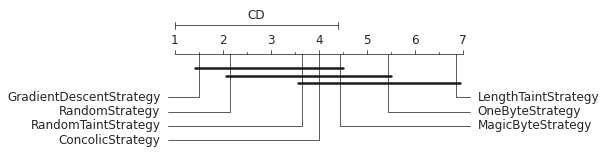
\includegraphics[width=0.8\textwidth]{5_results/graphs_new/cd_strategies.png}  
    \caption{Critical distance between average rank of the strategies.}
    \label{fig:cd-strategies}
\end{figure}

The strategies connected via a bold line are not statistically different from one another. The numbers shown are the average rank of the performance of the strategies, so closer to 1 means `first place' of a total of 7 positions.

Predictably, when we split the data between the OneByteStrategy and LengthTaintStrategy on one side and all other strategies on the other side, there is a significant difference between these groups. These strategies are rarely used, so they have the least amount of total flips. 
Interestingly enough, there is also a significant difference when we group the GradientDescentStrategy and RandomStrategy on the one side and the other strategies on the other side, which seems to confirm our results from Figure \ref{fig:overlap-strategies}.

We repeated this experiment but now replacing the flipped conditions found by the RandomStrategy by the conditions which were flipped which had taint information available. We obtained a p-value of $1.19 \cdot 10^{-4}$ by the Friedman test. The results are visible in Figure \ref{fig:cd-strategies-with-taint}.
\begin{figure}[H]
    \centering
    % include first image
    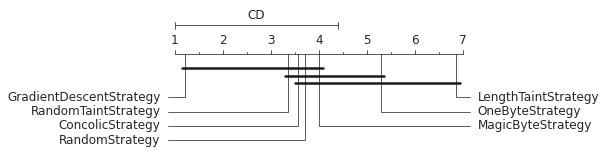
\includegraphics[width=0.8\textwidth]{5_results/graphs_new/cd_strategies_with_offset.png}  
    \caption{Critical distance between average rank of the strategies only considering tainted conditions.}
    \label{fig:cd-strategies-with-taint}
\end{figure}
We get somewhat similar results, but now it is clear that the GradientDescentStrategy is statistically different from all other strategies except the RandomTaintStrategy when considering only conditions which have taint information available.

\subsection{Time to flip}
The percentage of flipped conditions is not the only measure we have to compare the performance. We also measured the time a strategy spend mutating an input until a flip was found in a given condition. To compare the timing of the strategies, we rank the time a strategy took before a given condition was flipped for all conditions which have been flipped at least once. If a condition was never flipped by a strategy, we assign the maximum rank.
The mean ranks can be found in Figure \ref{fig:rank} the black lines are the confidence interval of 95\% of the data.
\begin{figure}[H]
    \centering
    % include first image
    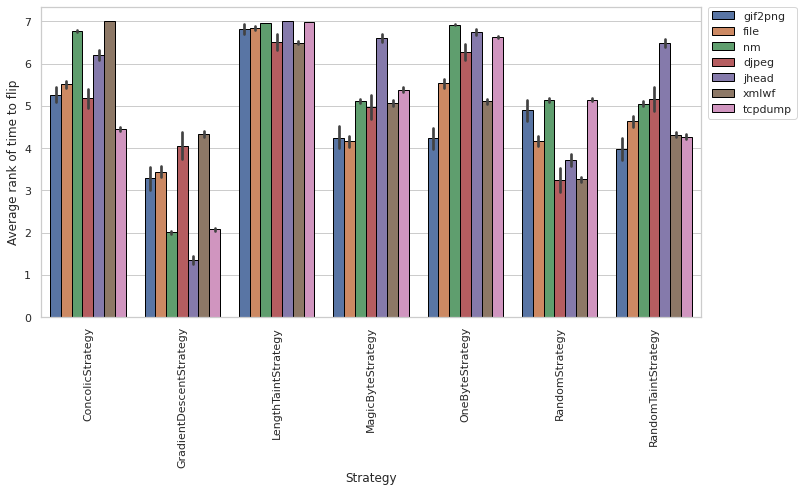
\includegraphics[width=1\textwidth]{5_results/graphs_new/ranks_with_time.png}  
    \caption{Average rank of the time to flip a condition per program}
    \label{fig:rank}
\end{figure}
Again the GradientDescentStrategy has the lowest rank and seems the fastest. 
We should watch out for data bias here, since there were a lot of flips found using the GradientDescentStrategy, it has more conditions where it was the only strategy which flipped the conditions, and this might skew the results.

We want to check if this result is also significant.
We have as null-hypothesis that there is no difference in the time to flip a condition between all strategies. If we perform a Friedmann test, we obtain a p-value of $3.34 \cdot 10^{-5}$, hence we reject our null-hypothesis with $\alpha = 0.05$, as we conclude that there is a significant difference between the strategies. Now we can perform a post-hoc Nemenyi test to see which individual strategies are significantly different from one another, again with  $\alpha = 0.05$. The results are visible in Figure \ref{fig:cd-strategies-with-rank}.
\begin{figure}[H]
    \centering
    % include first image
    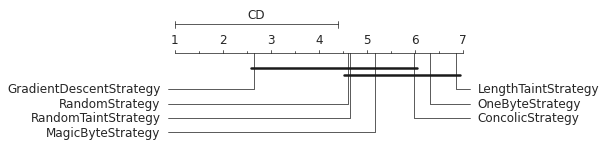
\includegraphics[width=0.8\textwidth]{5_results/graphs_new/CD_rank_timing.png}  
    \caption{Critical distance between average rank of the strategies only considering flipped conditions.}
    \label{fig:cd-strategies-with-rank}
\end{figure}
So here we see that there is a significant difference between the time of the GradientDescentStrategy against all other strategies.

\subsection{Substrategies}
We also looked at the used substrategies and their effectiveness.
We applied the strategies in the order as shown in Figure \ref{fig:substrategies}. If a condition was flipped by one substrategy, the next substrategy is not tried anymore. The results are shown in Figure \ref{fig:substrategies}.
We only look at flipped conditions, and using the MagicByteStrategy we see that the fill\_in substrategy is quite effective, just like the arithmatic substrategy which adds 1 byte. The zero extensions also seem to flips some extra conditions, but the encoding transformations do not seem to find a lot of extra flips.

The GradientDescendStrategy finds the same flips as the MagicByteStrategy due to the use of the substrategies, hence this strategy always outperform the other, and as additional bonus, it then picks a random starting point and restarts the GradientDescendStrategy from this input, where it repicks a random input when it is stuck in a local optimum. Hence this combines a part of the RandomTaintStrategy, and it shows that of all the flips found by this strategy at least 25\% and up to 70\% of all flips for the \texttt{tcpdump} binary are found using the random substrategy.
\begin{figure}[H]
    \centering
    % include first image
    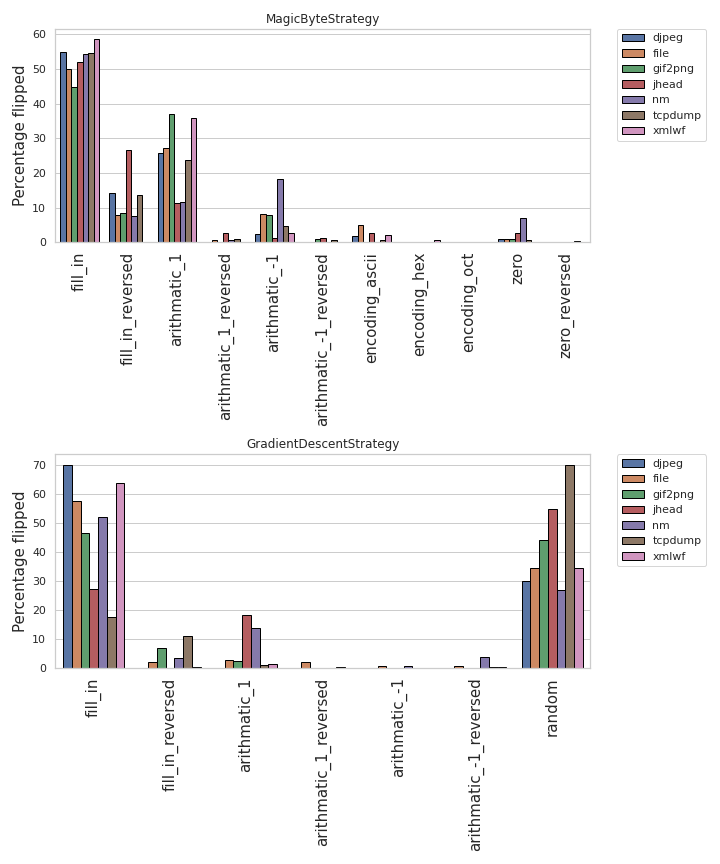
\includegraphics[width=0.8\textwidth]{5_results/graphs_new/substrategy_overview.png}  
    \caption{Distribution of flipped conditions by substrategy.}
    \label{fig:substrategies}
\end{figure}

\subsection{Microbenchmarks}
We also looked at the reasons why a strategy did not flip a condition. Here we see some expected results and some unexpected results.
The RandomStrategy is always tried, hence it can only be one of two reasons why it did not flip a condition, it either never reached the condition or it reached the conditions but the condition was not flipped. Only 15\% of the time did it never reach the condition, while in 85\% of the times it did reach the condition. The OneByteStrategy and LengthTaintStrategy are often never tried, as expected since these trigger only under special circumstances.
When we compare this with the RandomTaintStrategy, we see that it skips about 22\% of all cases, because there is no taint information available and of the tried inputs, over 50\% never reaches the condition it is trying to fuzz. The MagicByteStrategy reaches even less, over 60\% of the conditions are not reached.
Another curious case is the ConcolicStrategy, which apparently in about 58\% of the cases cannot generate any input for the condition.

\begin{figure}[H]
    \centering
    % include first image
    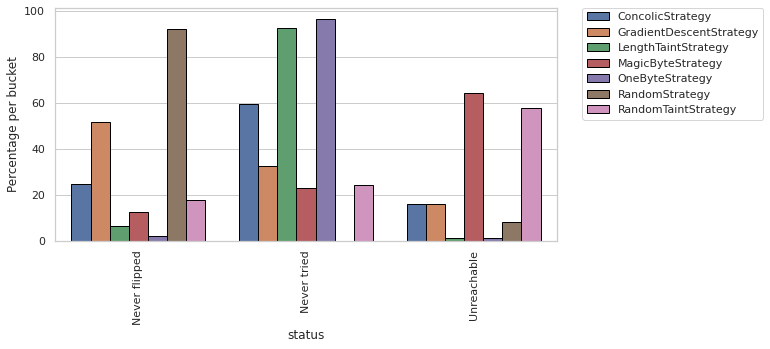
\includegraphics[width=0.8\textwidth]{5_results/graphs_new/benchmarks.png}  
    \caption{Distribution of not flipped conditions by micro-benchmark.}
    \label{fig:benchmarks}
\end{figure}

\subsection{Relation to metrics}
With some of the metrics we choose, we were not sure if this metric was helpful in providing any kind of information about the conditions. So the first thing we test is if we choose the right metrics. We want to know if there is a significant difference between the distribution of the metrics of the flipped conditions versus the distribution of the metrics of the non flipped conditions. If the relation between the metric and the flipped condition is independent, the distribution of the metric should be equal for flipped and not flipped conditions. However, if the metric is related to the result of the tried condition, the distribution should differ.
We perform a non-parametric Mann-Whitney U test \cite{metzman2020fuzzbench}, where the null hypothesis is that there is no difference in the distribution between the flipped and not flipped conditions. We want to look at the different distributions when we split the data per metric, but also per program. So we perform the test for every combination between metric and program. The results are visible in Figure \ref{fig:mann-whitney-program-metrics}.

\begin{figure}[H]
    \centering
    % include first image
    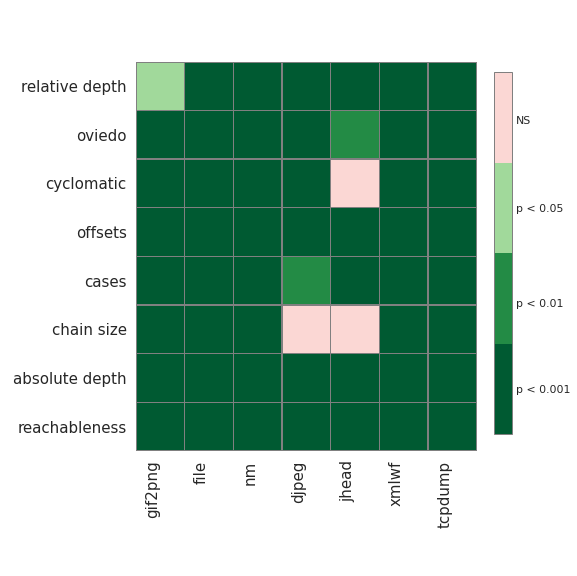
\includegraphics[width=0.8\textwidth]{5_results/graphs_new/mann_whitney_u_programs.png}  
    \caption{Results of the Mann-Whitney U test between programs and metrics}
    \label{fig:mann-whitney-program-metrics}
\end{figure}
Here we see that for any program, there is a significant difference in the distribution between the flipped and not flipped conditions for nearly all programs. Only the \texttt{djpeg} and \texttt{jhead} programs do not have a significant difference everywhere.

We are also interested in the difference between the strategies and the metrics, since this could be used to say which metric can predict the behaviour of a strategy. We again performed the test between every metric and strategy as shown in Figure \ref{fig:mann-whitney-strategy-metrics}.
\begin{figure}[H]
    \centering
    % include first image
    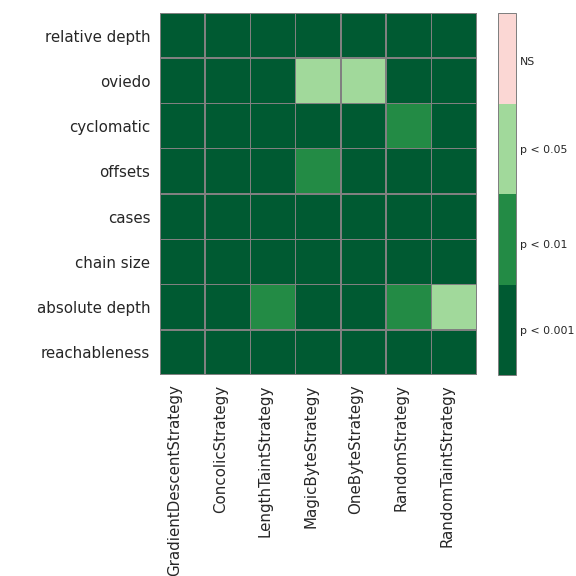
\includegraphics[width=0.8\textwidth]{5_results/graphs_new/mann_whitney_u_strategy.png}  
    \caption{Results of the Mann-Whitney U test between strategies and metrics}
    \label{fig:mann-whitney-strategy-metrics}
\end{figure}
We find that all metrics have a significant difference in the distribution between the flipped and not flipped conditions. 
This means that we should be able to differentiate between conditions which will be flipped and not be flipped based on our chosen metrics. In the next Section we will build a classifier which does this.

We further inspect the relation of the metrics with the strategies, now by focusing on our flipped conditions and the strategies which flipped the conditions.
We want to know when a metric results in the highest number of flips. For example, we expect that the number of flipped conditions decreases when the reachableness increases. However, we are also interested in the relation with the total time spend on a condition and the relative depth of the program when the condition was flipped.
We have constructed a kernel density estimation of where in the program, by looking at the relative depth, conditions where flipped in Figure \ref{fig:kde-relative}.

\begin{figure}[p]
    \centering
    % include first image
    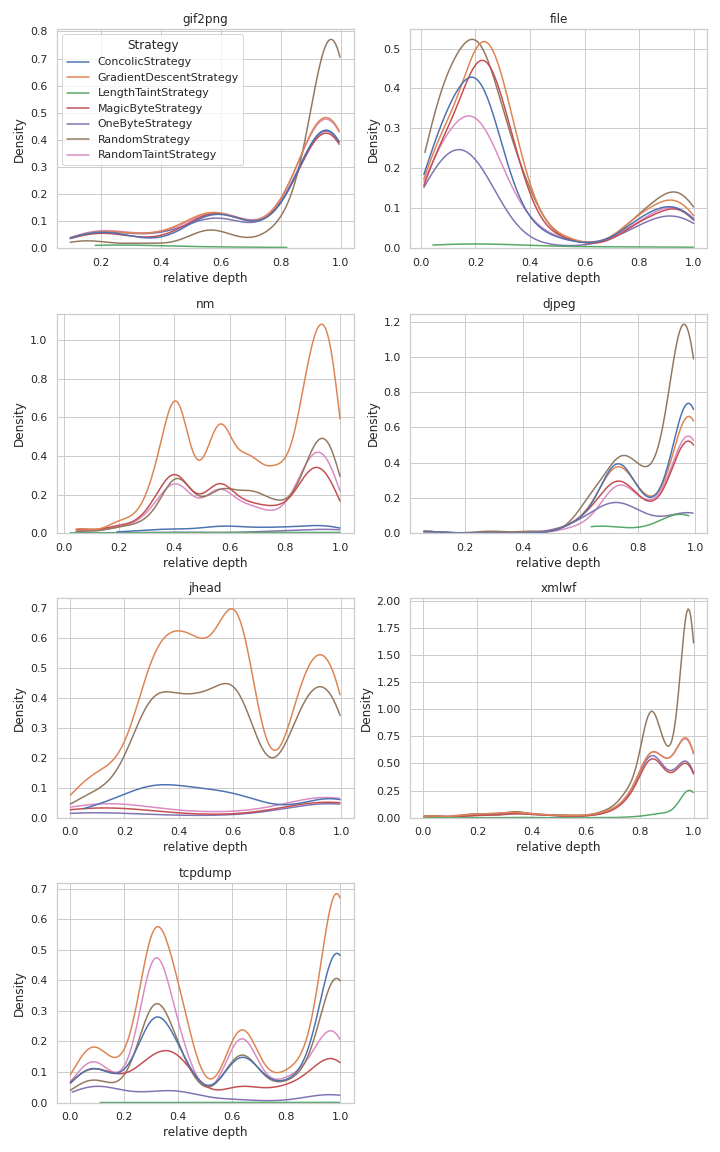
\includegraphics[width=0.9\textwidth]{5_results/graphs_new/kde_relative.png}  
    \caption{Kernel density estimation plots of the relative depth per program}
    \label{fig:kde-relative}
\end{figure}
We see that the depth where the conditions are flipped differs between programs. Some programs have more flipped conditions at the end, like \texttt{gif2png} and \texttt{xmlwf}, while other like \texttt{jhead} seem to find more flipped conditions in the middle. It looks like there are some `hotspots' in the programs where more conditions are flipped than in other locations. 

Another notable result, is that most strategies are grouped together, when one strategy finds flipped conditions, others also find flipped conditions at the same locations.
%In the \texttt{jhead} binary, it is visible that the GradientDescentStrategy outperforms the other strategies, but also the RandomStrategy outperforms the other strategies here.

The reachableness metric is shown in Figure \ref{fig:kde-reachableness} with a cutoff at 200, since there were some extreme values. Here the strategies also seem to follow one another closely for some programs, for example in the \texttt{gif2png} binary, or with distinct peaks in the \texttt{jhead} binary. The plots confirm our suspicion, most flipped conditions occur when the reachability is low, hence there are not many bytes compared in the conditions or before the condition. This means this is likely a good metric to include in our models.

%We have shown that for some variables, the graphs look cautiously optimistic when looking for a relation.

\begin{figure}[p]
    \centering
    % include first image
    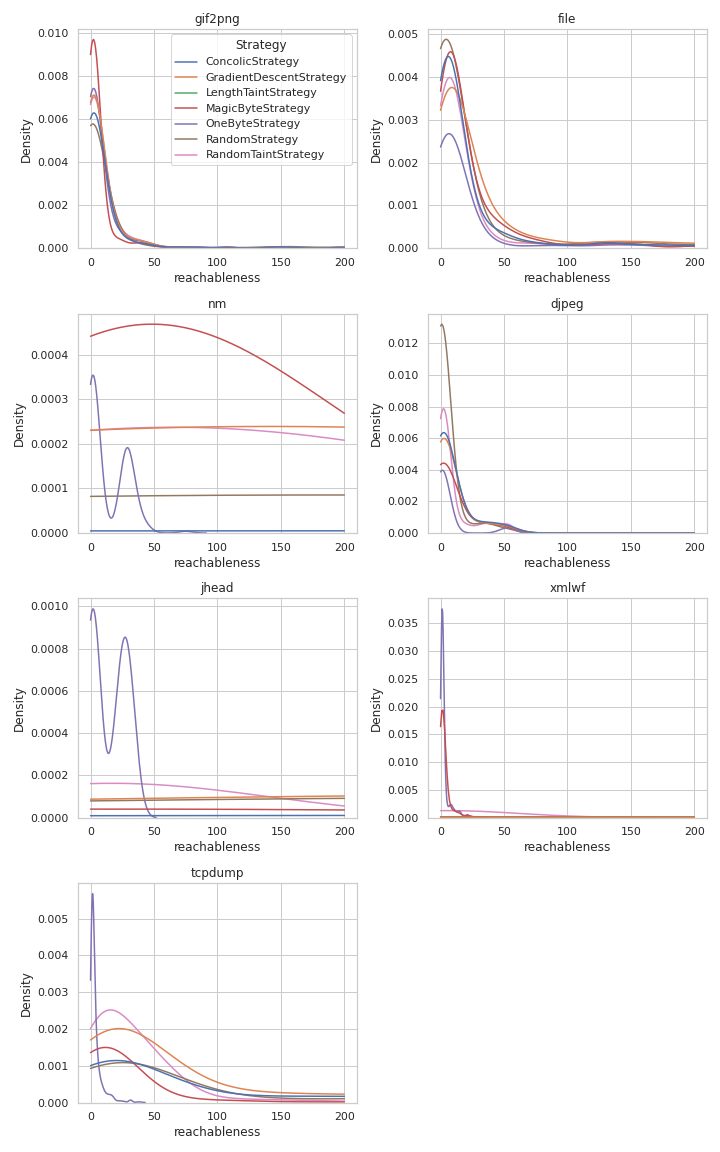
\includegraphics[width=\textwidth,height=\textheight,keepaspectratio]{5_results/graphs_new/kde_reachableness.png}  
    \caption{Kernel density estimation plots of reachableness per program}
    \label{fig:kde-reachableness}
\end{figure}

Another important measure of performance is the time a strategy has spend on a condition. We again look at a kernel density estimation plot with the time on a logarithmic scale. We plotted the time on a logarithmic scale, since a lot of flipped conditions take a fraction of a second, while others take over 10 seconds.
We see that a lot of strategies manage to finish within a second, but some strategies take longer, like the RandomStrategy which also has a peak a little before 15 seconds. This is possibly due to the multiple runs of this strategy, where if one run manages to flip a condition, we still take the average time. If other runs did not manage to find a flip, those runs timeout at 15 seconds. Hence the average lays close to 15. It is notable that other strategies often find the flip within the first second, even the more advanced strategies like the GradientDescentStrategy.
Since there is so much data in the first second, where the differences are small, we expect that predicting the fastest strategy with machine learning models can be a problem.


\begin{figure}[H]
    \centering
    % include first image
    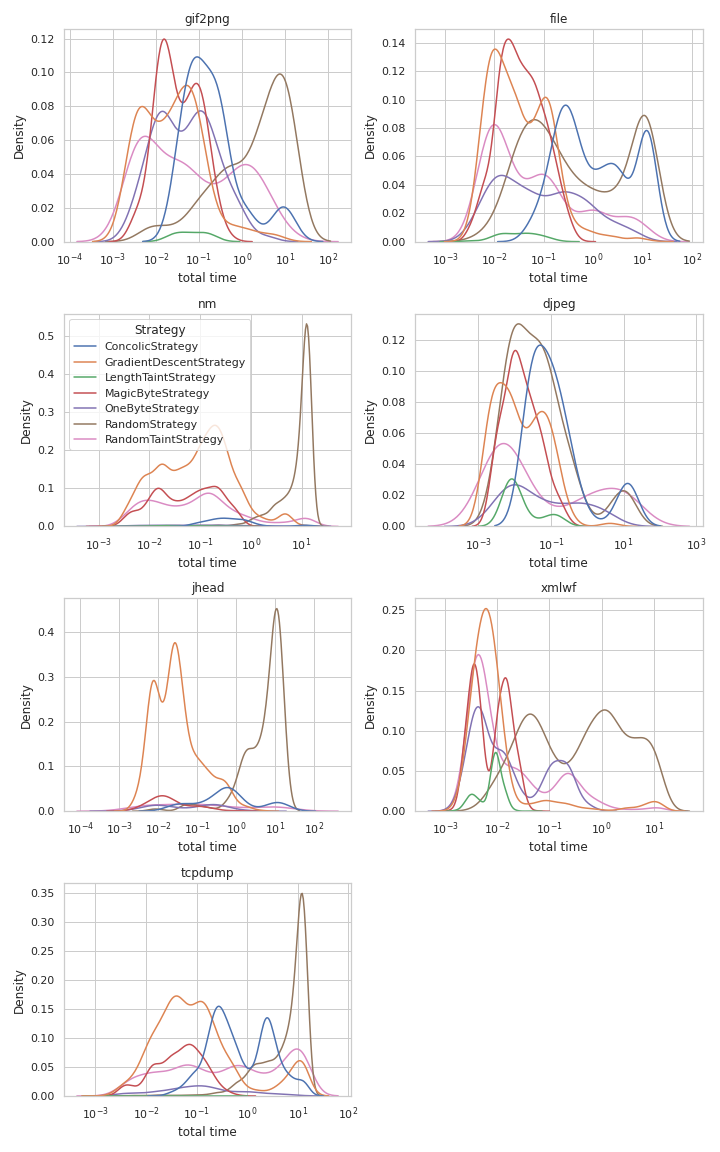
\includegraphics[width=\textwidth,height=\textheight,keepaspectratio]{5_results/graphs_new/kde_flipped_timing.png}  
    \caption{Kernel density estimation plots of total time per program}
    \label{fig:kde-timing}
\end{figure}

From the timing plots, we see interesting behaviour of the ConcolicStrategy, which appears to be done within the time limit. We found that the ConcolicStrategy needs on average $1.85$ seconds to flip a branch when offsets are available, while it takes on average $10.59$ seconds when no offset information is available. This shows that a combination of dynamic taint analysis and symbolic execution can increase the average speed of a symbolic strategy nearly tenfold. This is shown in Table \ref{tab:concolic-info}.

\begin{table}[H]
\centering
\begin{tabular}{l|rr}
\toprule
Strategy &  Offsets available &  No offsets available \\
\midrule
count &            6287 &                118 \\
mean  &               1.85 &                 10.59 \\
std   &               3.00 &                  5.06 \\
min   &               0.02 &                  0.04 \\
25\%   &               0.23 &                 11.81 \\
50\%   &               0.48 &                 13.09 \\
75\%   &               2.31 &                 13.23 \\
max   &              14.98 &                 14.98 \\
\bottomrule
\end{tabular}

\caption{Timing information of the ConcolicStrategy where a condition was flipped}\label{tab:concolic-info}
\end{table}

Other plots are less interesting and can be found in Figure \ref{fig:kde-flipped-conditions}. An unexpected result is that most strategies seem to find flips for the same metrics, except the LengthStrategy.

%After this analysis, we can create models with the goal of predicting properties of a condition with only the metrics as input.

\section{Creating models}
In the previous Section, we found that some strategies seem to outperform others when looking at the overall performance. However, we also found a significant difference between the distribution of the flipped and not flipped conditions when comparing different strategies and metrics. So we create models as explained in Section \ref{sec:overview}. In the field of machine learning, the collected metrics are called features. To be consistent in this naming convention we will refer to the individual metrics in this Section by calling them features.

\subsection{Feature selection}
The first step in our model creation is the selection of the right features.
Not all features are important when creating the models and some features can be correlated with one another. We filter the features which have a high correlation and analyse which of the remaining features are more important than others.

To calculate the correlation, we use Spearman's rank correlation coefficient \cite{lehman2005jmp} as shown in Figure \ref{fig:correlation}. Here we calculate this coefficient for every program separately for every combination of features.
\begin{figure}[p]
    \centering
    % include first image
    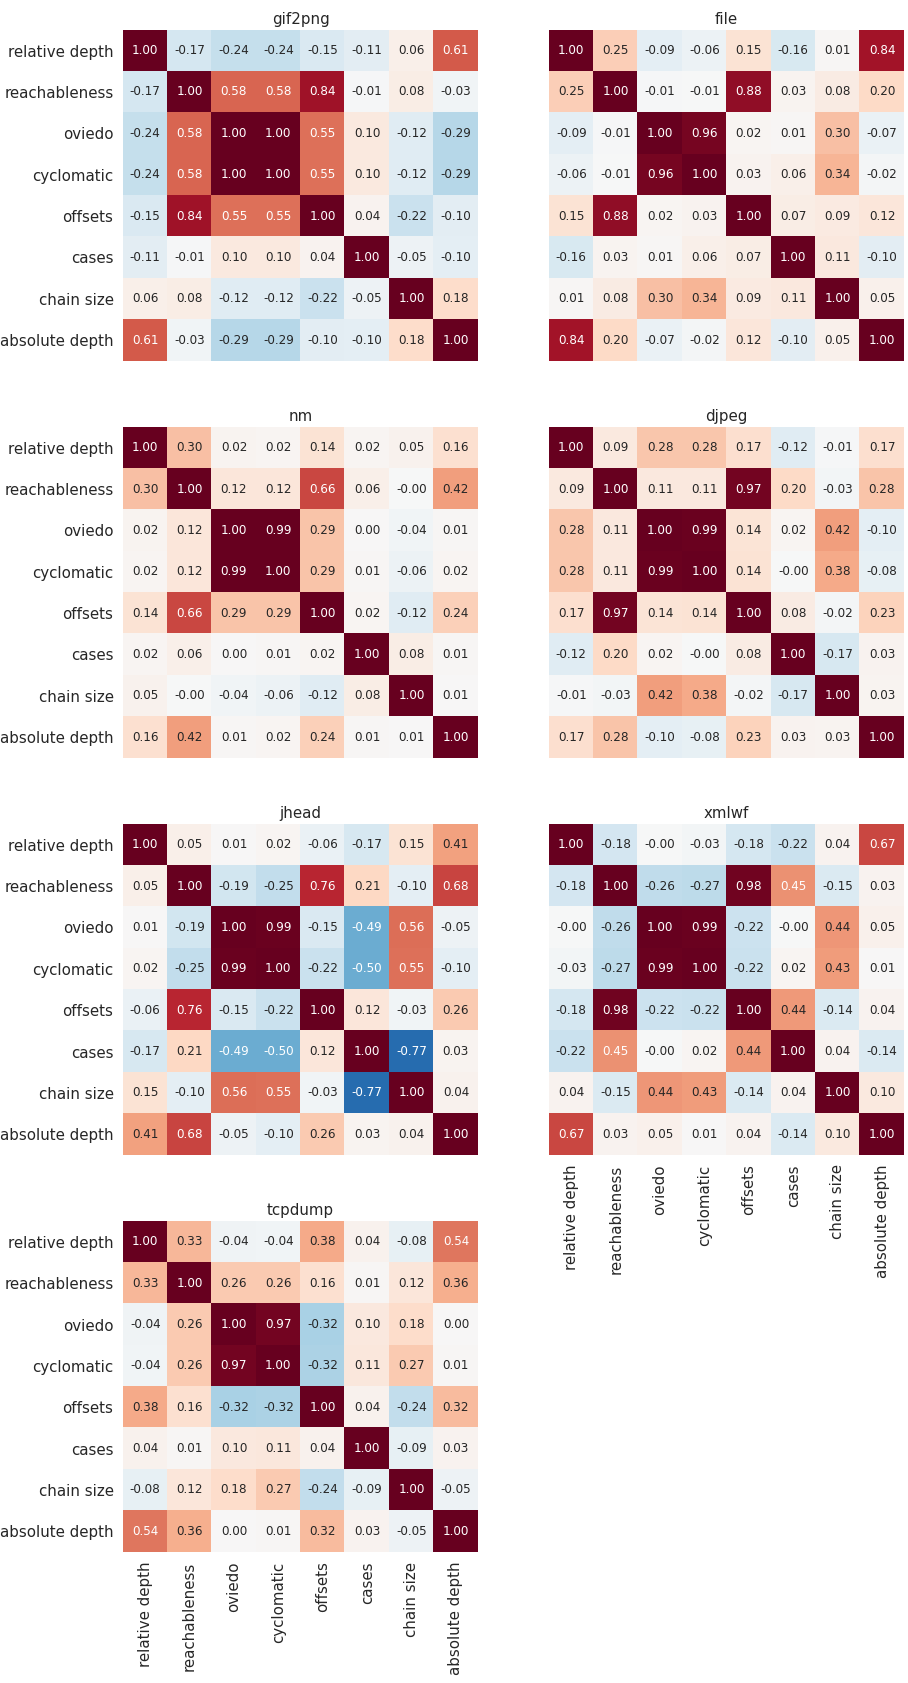
\includegraphics[height=\textheight]{5_results/graphs_new/correlation_benchmarks.png}  
    \caption{Heatmap of correlation coefficients between all features per program}
    \label{fig:correlation}
\end{figure}
We see that the Oviedo and the cyclomatic complexity are highly correlated, nearly one-on-one. We also notice that the reachableness and offsets are highly correlated, since the reachableness metric is more specific case of the offsets metric, however not in all cases.

Our next step is calculating the mutual information for every feature and the flipped conditions. When this value equals 0, it means that the variables are independent, so they cannot be related to one another, higher values indicate that it can be used to estimate if a condition can be flipped. The results are displayed in Figure \ref{fig:feature-importance}.

\begin{figure}[H]
    \centering
    % include first image
    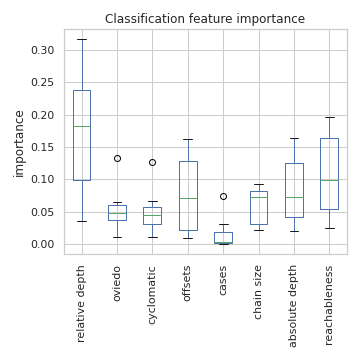
\includegraphics[width=0.5\textwidth]{5_results/graphs_new/feature_selection.png}  
    \caption{Mutual information per feature for the flipped conditions}
    \label{fig:feature-importance}
\end{figure}

We see that the relative depth has the highest average importance, and the cases feature often is of very low importance. The offsets and reachablesness are also important features, and Oviedo complexity and the chain size are not the highest, but we still include them. This gives us the selected features: relative depth, Oviedo complexity,  offsets, chain size and reachableness. We disregard the absolute depth metric, because we already have the relative depth, and the absolute depth has a lower importance than the relative depth.

For the model which predicts the time, we have to look at the mutual information between the selected features and the total time while considering only the flipped conditions. The results are given in Figure \ref{fig:feature-importance-regressor}.

\begin{figure}[ht]
    \centering
    % include first image
    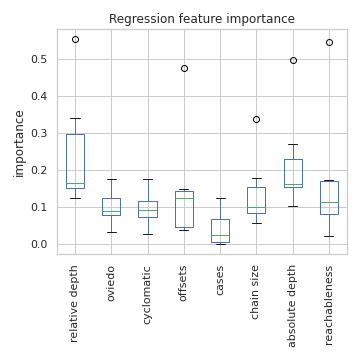
\includegraphics[width=0.5\textwidth]{5_results/graphs_new/feature_selection_regression.png}  
    \caption{Mutual information per feature for the total time}
    \label{fig:feature-importance-regressor}
\end{figure}

We notice that the results are pretty similar, except that the absolute depth feature is more important than before, however, the relative depth has a slightly higher average, hence our selection of features does not change.

\subsection{Predicting flipped conditions}
To create a model which classifies a condition as flippable or not flippable, we train a number of machine learning models and assess their performance using the metrics described in Section \ref{sec:MLmodels}. We also try to find the best parameters by using 5-fold cross validation. To perform cross validation, the data is randomly split in a test set of 40\% and a training set of 60\% of the original data.
In Table \ref{tab:classifiers-overview} we give an overview of the tested models and the search space for their hyperparameters.
To see if it actually performed better, we also compared it using a DummyClassifier for every program. A DummyClassifier just returns the most frequent label from the training data, no mater what input is given.

In Table \ref{tab:classifiers-result} we show the best scores per model including the comparison with the DummyClassifier. We quickly notice that the DecisionTreeClassifier (DT) is in all cases the best model, except for the \texttt{gif2png} and \texttt{jhead} binary and that the DummyClassifier is outperformed everywhere.
\begin{table}[H]
\centering
\begin{tabular}{lllll}
\toprule
{} &        Best precision &           Best recall &         Best f1-score &         Best accuracy \\
\midrule
gif2png &  0.700 (DT) &       0.685 (Gausian) &       0.687 (Gausian) &       0.685 (Gausian) \\
file    &  0.902 (DT) &  0.903 (DT) &  0.902 (DT) &  0.903 (DT) \\
nm      &  0.840 (DT) &  0.840 (DT) &  0.840 (DT) &  0.840 (DT) \\
djpeg   &  0.860 (DT) &  0.855 (DT) &  0.857 (DT) &  0.855 (DT) \\
jhead   &           0.843 (SVC) &           0.843 (SVC) &           0.843 (SVC) &           0.843 (SVC) \\
xmlwf   &  0.808 (DT) &  0.807 (DT) &  0.807 (DT) &  0.807 (DT) \\
tcpdump &  0.836 (DT) &  0.836 (DT) &  0.836 (DT) &  0.836 (DT) \\
\bottomrule
\end{tabular}

\caption{Models which scored the highest per scoring metric.}\label{tab:classifiers-result}
\end{table}
We achieve relatively good scores of slightly above 80\% accuracy and precision for most programs, except the \texttt{gif2png} binary. 
%Since we use a DecisionTreeClassifier, we can actually look at the decision tree and how the classifier is constructed as shown in Figure \ref{fig:decision-tree-gif2png}.
\begin{comment}
\todo{does this contribute to the paper?}
\begin{figure}[h]
    \centering
    % include first image
    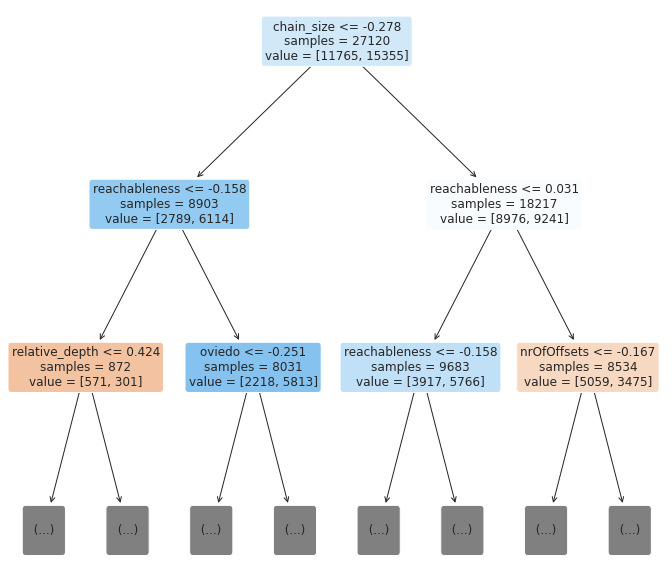
\includegraphics[width=\textwidth,height=\textheight,keepaspectratio]{5_results/graphs_new/decision_tree.png}  
    \caption{Part of the decision tree of the \texttt{gif2png} binary.}
    \label{fig:decision-tree-gif2png}
\end{figure}
\end{comment}

We also recreated the models but now we used Principal Component Analysis (PCA) in order to reduce the number of features by transforming the data to a space where every column is orthogonal to the previous columns when interpreting the columns like vectors. Using this technique, we could explain 95\% of the variance variance with only 3 columns in our transformed dataset. However, the created classifiers performed overall, worse than the previous created classifiers. The results are shown in Table \ref{tab:classifiers-result-pca}.

\begin{table}[H]
\centering
\begin{tabular}{lllll}
\toprule
{} &        Best precision &           Best recall &         Best f1-score &         Best accuracy \\
\midrule
gif2png &           0.702 (SVC) &           0.705 (SVC) &           0.697 (SVC) &           0.705 (SVC) \\
file    &  0.832 (DT) &  0.831 (DT) &  0.831 (DT) &  0.831 (DT) \\
nm      &  0.688 (DT) &  0.688 (DT) &  0.688 (DT) &  0.688 (DT) \\
djpeg   &  0.806 (DT) &  0.801 (DT) &  0.803 (DT) &  0.801 (DT) \\
jhead   &       0.840 (Gausian) &       0.850 (Gausian) &  0.833 (DT) &       0.850 (Gausian) \\
xmlwf   &  0.757 (DT) &  0.751 (DT) &  0.753 (DT) &  0.751 (DT) \\
tcpdump &  0.764 (DT) &  0.765 (DT) &  0.764 (DT) &  0.765 (DT) \\
\bottomrule
\end{tabular}

\caption{Models which scored the highest per scoring metric after PCA.}\label{tab:classifiers-result-pca}
\end{table}
We note however, that these models were trained after the fuzzing runs were already performed. When we compare the constructed models of the programs between one another, the accuracy reaches 0.5, where it becomes no more powerful than a coin toss. Hence, if a fuzzer would use this approach, it would need to train the model during the fuzzing run for a specific program.

\subsection{Predicting time spend}
The next step is creating a model which tells us which strategy we should use when we find a flippable condition. We should pick a strategy which flips the condition the fastest. We can do this in one of two ways. We either create another classifier which predicts for a condition the fastest strategy, or we create a regression model to predict the time spend on a condition by a strategy and then select the strategy which is predicted to be the fastest. We should only select conditions where a flip occurs.

When using the classifier models as we did previously, we run into the problem that some strategies, or labels, only occur very infrequent in the results, which results in poor results when using 5-fold cross validation. When we compared the created classifiers with a DummyClassifier, this outperformed the created models for every program for every scoring metric. Hence we choose to create a regression model.

We again try a number of different regression models and estimate the best parameters using 5-fold cross validation. The tested models and the search space for the hyperparameters can be found in Table \ref{tab:regressor-overview}. The scores of the median average error seem to be rather low, they are all well under 1 second, which looks promising.
To see if the results make sense, we compare them to a DummyRegressor. This model just returns the median total time for every strategy.
When looking at the DummyRegressor, the median absolute error is also well below 1 second for all programs. We even see that the DummyRegressor outperforms the other models for the \texttt{nm} binary. This leads us to believe that these models do not predict the most optimal strategy since without any features the predictions are also very close. So the constructed models cannot be used to accurately predict the time spend.
When we try to use one model to predict the results of the other models, the results become way worse. We obtained an MAE of $2.800$ when comparing the model for the \texttt{gif2png} binary with the data of all other programs. Hence, the constructed models are not portable, and should be reconstructed per program during a fuzzing run.
\begin{table}[H]
\centering
\begin{tabular}{lll}
\toprule
{} &             Best model &         MAE \\
\midrule
gif2png &  DecisionTreeRegressor &     0.46247 \\
file    &  DecisionTreeRegressor &   0.0990765 \\
nm      &         DummyRegressor &   0.0567867 \\
djpeg   &  DecisionTreeRegressor &  0.00896336 \\
jhead   &  DecisionTreeRegressor &    0.222155 \\
xmlwf   &  DecisionTreeRegressor &     0.04854 \\
tcpdump &  DecisionTreeRegressor &    0.326539 \\
\bottomrule
\end{tabular}

\caption{Models which scored the lowest Median Absolute Error}\label{tab:regressor-result}
\end{table}

To see if we performed better when transforming the data using PCA, we trained our models again. We now no longer underperfom the DummyRegressor, but in 4 of the 7 programs we perform worse than the untransformed results. The results can be seen in Table \ref{tab:regressor-result-pca}. 
\begin{table}[H]
\centering
\begin{tabular}{lll}
\toprule
{} &             Best model &        MAE \\
\midrule
gif2png &  DecisionTreeRegressor &   0.371041 \\
file    &  DecisionTreeRegressor &  0.0732656 \\
nm      &              LinearSVR &  0.0494515 \\
djpeg   &  DecisionTreeRegressor &  0.0143483 \\
jhead   &  DecisionTreeRegressor &   0.249539 \\
xmlwf   &              LinearSVR &  0.0737347 \\
tcpdump &  DecisionTreeRegressor &   0.385287 \\
\bottomrule
\end{tabular}

\caption{Models which scored the highest per scoring metric after PCA.}\label{tab:regressor-result-pca}
\end{table}
These results show that it is very hard to predict which strategy manages to flip a condition faster than another strategy by using our collected features.